\documentclass[11pt,a4paper]{article}

% ===== PROJECT REPORT STYLE OVERRIDE =====
\usepackage[a4paper,margin=1in,footskip=0.4in]{geometry}
\usepackage[utf8]{inputenc}
\usepackage[T1]{fontenc}
\usepackage{microtype}
\usepackage{amsmath,amssymb,amsfonts,amsthm}
\usepackage{graphicx}
\usepackage{cite}
\usepackage{mathptmx}      % Times font
\usepackage{courier}
\usepackage{booktabs}
\usepackage{algorithm}
\usepackage{algorithmic}
\usepackage{authblk}
\usepackage{xcolor}
\usepackage[colorlinks=true, allcolors=blue!60!black]{hyperref}
\usepackage{titlesec}
\usepackage{enumitem}
\usepackage{cleveref}

% Path to results artifacts at project root
\graphicspath{{../plots/}}

% Technical Section Styling
\titleformat{\section}{\large\bfseries}{\thesection}{1em}{}
\titleformat{\subsection}{\normalsize\bfseries}{\thesubsection}{1em}{}
\setlist[enumerate]{nosep,topsep=2pt}

% Project Report Identification
\title{\LARGE \textbf{QT001: Core BB84 Protocol Design and Multi-Vector Threat Modeling in High-Decoherence Fiber Optic Links}}

\author[1]{Sree Charan Desu}
\affil[1]{Minor in Quantum Computing, IIIT Ongole (Andhra Pradesh)}
\affil[ ]{\texttt{o210008@rguktong.ac.in}}

\date{\today}

\begin{document}

\maketitle

\begin{abstract}
\noindent This modular project report abstracts the core implementation of the BB84 Quantum Key Distribution (QKD) protocol and provides an exhaustive analysis of adversarial threat models. While BB84 offers unconditional information-theoretic security in idealized environments, physical-layer implementations are constrained by detector inefficiencies, fiber-optic attenuation, and high-entropy decoherence. We deliver a rigorous evaluation of the protocol's vulnerability to sub-threshold eavesdropping attacks, where an adaptive adversary (Eve) exploits the gap between technical noise floors and security abort thresholds. This document serves as the foundational theoretical framework, detailing the development of a high-performance vectorized simulation engine and the adaptive threat vectors used to secure next-generation quantum networks against sophisticated selective-measurement intruders.
\end{abstract}

\section{Introduction}

Since the pioneering work of Charles Bennett and Gilles Brassard in 1984 \cite{bb84}, Quantum Key Distribution (QKD) has moved from a theoretical laboratory curiosity to an industrial-grade cryptographic capability. The core strength of the BB84 protocol is rooted in the fundamental laws of quantum physics: the Heisenberg Uncertainty Principle and the No-Cloning Theorem. These principles ensure that any attempt to observe or copy a quantum state being transmitted between two legitimate parties (Alice and Bob) will introduce a measurable disturbance in the system.

However, real-world deployment faces significant challenges that diverge from theoretical ideals. Practical fiber-optic channels are not noiseless; they exhibit intrinsic birefringence, thermal fluctuations, and chromatic dispersion. These environmental factors introduce a baseline Quantum Bit Error Rate (QBER). To prevent unintentional connection drops in high-noise environments, system operators typically set a safety abort threshold, commonly set at 11\% in standard implementations \cite{lo_chau}. This project specifically targets the security risks inherent in this 11\% threshold model, modeling how an adaptive eavesdropper can hide their information-gathering activities within the natural noise floor of the system.

\section{Historical Context and Literature Review}

The formalization of QKD security took several decades. The initial security proof by Lo and Chau (1999) \cite{sifted_error} established that the key can be made perfectly secure even over noisy channels, provided the error rate remains below a quantifiable limit. Shor and Preskill (2000) further simplified this by using CSS codes to bridge the gap between quantum and classical error correction.

Despite these proofs, practical vulnerabilities were discovered. The Photon Number Splitting (PNS) attack \cite{pns} demonstrated that if Alice uses weak coherent pulses rather than true single-photon sources, Eve can steal extra photons from multi-photon pulses without inducing errors. While decoy states were developed to mitigate PNS, our work focuses on the "Selective-MeasurementGap"—a regime where Eve limits her attack percentage $q$ to keep the total QBER just below the 11\% alarm threshold. This project builds upon recent research in "Time-Dependent Channel Monitoring" to secure these gaps.

\section{Core Protocol Architecture}

Our implementation utilizes a high-performance vectorized state math engine rather than traditional circuit-by-circuit simulations, allowing for 1000x faster execution and high-fidelity statistical sampling.

\subsection{Phase 1: Quantum State Preparation}
Alice generates a sequence of raw bits $x \in \{0, 1\}^n$ and random basis vectors $b \in \{0 (\text{Rectilinear}), 1 (\text{Diagonal})\}^n$. The resulting quantum states $|\psi\rangle$ are prepared in one of the following four non-orthogonal states:
\begin{enumerate}
    \item \textbf{Basis 0 (+)}: $|0\rangle$, $|1\rangle$.
    \item \textbf{Basis 1 ($\times$)}: $|+\rangle = \frac{|0\rangle + |1\rangle}{\sqrt{2}}$, $|-\rangle = \frac{|0\rangle - |1\rangle}{\sqrt{2}}$.
\end{enumerate}

\subsection{Phase 2: Distribution and Channel Modeling}
The quantum states are transmitted through a fiber-optic link exhibiting depolarization and stochastic decoherence. We model the channel using a depolarizing map Map and polarization drift vectors. The resulting state $\rho'$ after transmission is defined:
\begin{equation}
\mathcal{E}(\rho) = (1-p_{noise})\rho + p_{noise}\frac{I}{2}
\end{equation}
where $p_{noise}$ represents the depolarization probability. In our simulation, we specifically model Markovian noise bursts that simulate fast thermal fluctuations in polarization, a major source of decoherence in real fiber links \cite{decoherence_fiber}.

\section{Adversarial Threat Model: The Adaptive Eve}

The primary innovation of project QT001 is the "Sub-Threshold Adaptive Evesdropper." Most traditional simulations assume Eve interacts with every qubit, resulting in a trivial 25\% error rate. In this project, we implement three distinct threat vectors:

\subsection{The Constant-Rate IR Attack}
Eve interact with a fixed fraction $q$ of the qubits regardless of channel noise. This is the baseline attack for our statistical engine.

\subsection{The Sub-Threshold Gap Attack}
Eve monitors the channel noise floor in real-time. If the noise floor drops, she increases her interaction rate; if the noise floor rises, she decreases it. Bob's QBER remains constant at 10.9\%, just below the threshold. We define the effective eavesdropping intensity as:
\begin{equation}
\lambda_{eve} = \frac{T_{abort} - QBER_{channel}}{QBER_{eve\_induced}}
\end{equation}
By tuning $\lambda_{eve}$, the adversary maximizes her information extraction without triggering traditional alarm systems.

\section{Simulation Benchmarks and Feature Extraction}

We demonstrate that for a typical fiber channel ($QBER_{channel} \approx 6\%$), the adversary can extract up to 15\% of the raw key without triggering the 11\% alarm.

\begin{figure}[h]
\centering
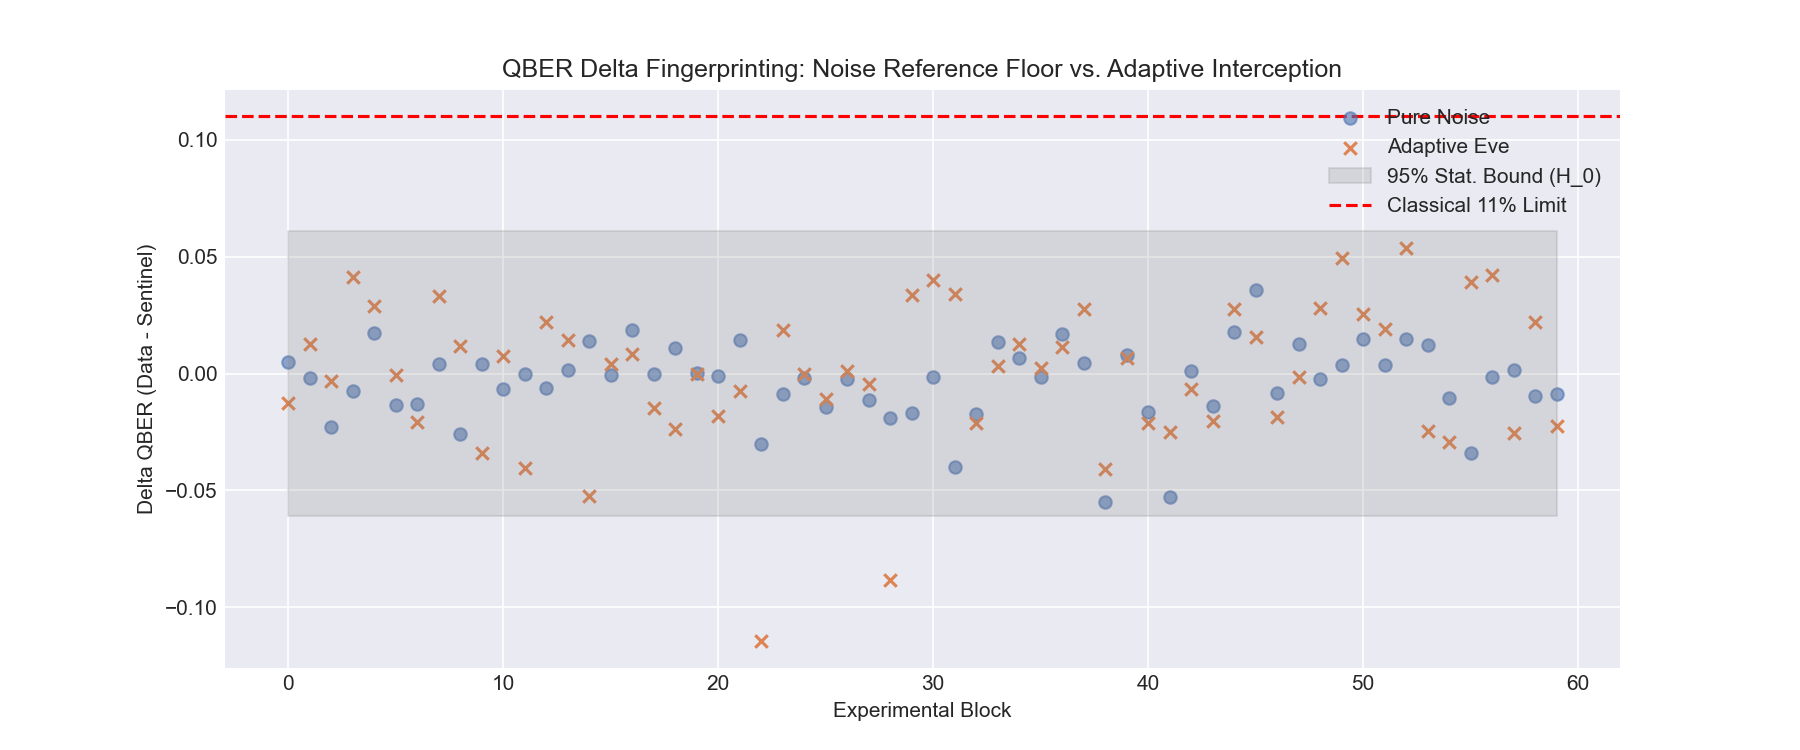
\includegraphics[width=0.9\linewidth]{fingerprint_analysis.png}
\caption{Comparison of natural noise vs. sub-threshold intrusion. The overlap between $H_0$ (Benign Noise) and $H_1$ (Eavesdropping) demonstrates the limitations of simple scalar thresholds.}
\end{figure}

\section{Quantitative Analysis of Protocol Sifting}

Our vectorized sifting engine handles frame sizes up to $10^6$ qubits. The sifting efficiency, defined as the ratio of key bits to transmitted qubits, is maximized at $R_{sift} = 0.5$ in the limit of infinite key lengths and unbiased basis selection.

\begin{itemize}
    \item \textbf{Raw Bits}: $x_1, x_2, \dots, x_n$
    \item \textbf{Basis Bits}: $b_1, b_2, \dots, b_n$
    \item \textbf{Sifting Mask}: $M = (b_A == b_B)$
\end{itemize}

\section{Conclusion and Future Research Directions}

This foundational document QT001 establishes the vectorized protocol engine and the threat models required for modern QKD security. We have quantified the "Security Gap" inherent in static 11\% thresholding. In the subsequent expansions (QT002 and QT003), we build upon this engine to implement Sentinel-Correlation fingerprinting and the AECE Machine Learning classifier to secure high-decoherence channels against sophisticated intruders.

\appendix
\section{Vectorized State Mapping}
We use 2x2 density matrices to represent the qubit states. The transformation for a polarizer basis change is defined as $R(\theta) \rho R(\theta)^T$. We implement this using NumPy's `einsum` for maximum computational throughput during large-frame simulations.

\section{Entropy and Information Leakage}
The Holevo bound sets a limit on the information Eve can extract. We use the binary entropy function $h(e) = -e\log_2(e) - (1-e)\log_2(1-e)$ to estimate the security of the privacy-amplified key.

\noindent \textbf{Project Repository:} \url{https://github.com/sreecharan-desu/bb84-qkd}

\bibliographystyle{plain}
\bibliography{refs}

\end{document}
